\documentclass[10pt,a4paper]{article}
\usepackage[utf8]{inputenc}
\usepackage{amsmath}
\usepackage{amsfonts}
\usepackage{multicol}
\usepackage{amssymb}
\usepackage[framed]{matlab-prettifier}
\usepackage{graphicx}
\usepackage[margin=0.75in]{geometry}
\usepackage{enumerate}
\usepackage{circuitikz}
\usepackage[utf8]{inputenc}
\usepackage[T1]{fontenc}
\usepackage{karnaugh-map}
\usepackage{tikz}
\usetikzlibrary{shapes.gates.logic.US}
\usetikzlibrary{circuits.ee.IEC}

\begin{document}
\begin{center}

{\huge EE5811 : FPGA LAB}\\
{\large ASSIGNMENT 1}

\end{center}
Rubeena Aafreen \hfill EE20RESCH11012

\vspace{15pt}
\hrule
\vspace{5pt}
\section{Problem}
Derive a Canonical SOP expression for a Boolean function $F$, represented by the following truth table

\begin{center}
    \begin{table} [h!]
    \centering
    \begin{tabular}{ | c | c | c | c | }
    \hline
    A & B & C & F(A,B,C) \\ [0.5ex]
     \hline
    0 & 0 & 0 & 1 \\
    0 & 0 & 1 & 0 \\
    0 & 1 & 0 & 0 \\
    0 & 1 & 1 & 1 \\
    1 & 0 & 0 & 1 \\
    1 & 0 & 1 & 0 \\
    1 & 1 & 0 & 0 \\
    1 & 1 & 1 & 1 \\ [1ex]
    \hline
    \end{tabular}
    \end{table}
\end{center}
\vspace{15pt}
\hrule
\vspace{5pt}

\section{Solution}
\subsection{KMAP Implementation}
\begin{figure}[!ht]
\centering
{
\begin{karnaugh-map}[4][2][1][][]
    \minterms{0,3,4,7}
    \maxterms{1,2,5,6}
    \implicant{0}{4}
    \implicant{3}{7}
    \draw[color=black, ultra thin] (0,2) --
    node [pos=0.7, above right, anchor=south west] {$BC$} % YOU CAN CHANGE NAME OF VAR HERE, THE $X$ IS USED FOR ITALICS
    node [pos=0.7, below left, anchor=north east] {$A$} % SAME FOR THIS
    ++(135:1);
    \end{karnaugh-map}
}
\caption{SOP for F using KMAP}
\label{fig1}
\end{figure}
The given expression can be minimized using KMap as shown in Figure \ref{fig1}. Using implicants in figure, SOP terms obtained are: $\Bar{B}\Bar{C}+BC$\\
\subsection{Minimized SOP Expression}
\begin{align}
    F=BC+\Bar{B}\Bar{C}
\end{align}
\subsection{NAND Expression}
To express the given SOP expression using NAND gates, we have
\begin{align}
    &F(A,B,C)=BC+\Bar{B}\Bar{C}\\
    &F(A,B,C)=\overline{(\overline{BC+\Bar{B}\Bar{C}})}\\
    &F(A,B,C)=\overline{(\overline{BC} . \overline{\Bar{B}\Bar{C}})}
\end{align}
\newpage
\subsection{NAND Gate Implementation}
Circuit diagram with NAND gates is shown below:
\begin{figure}[ht!]
\centering
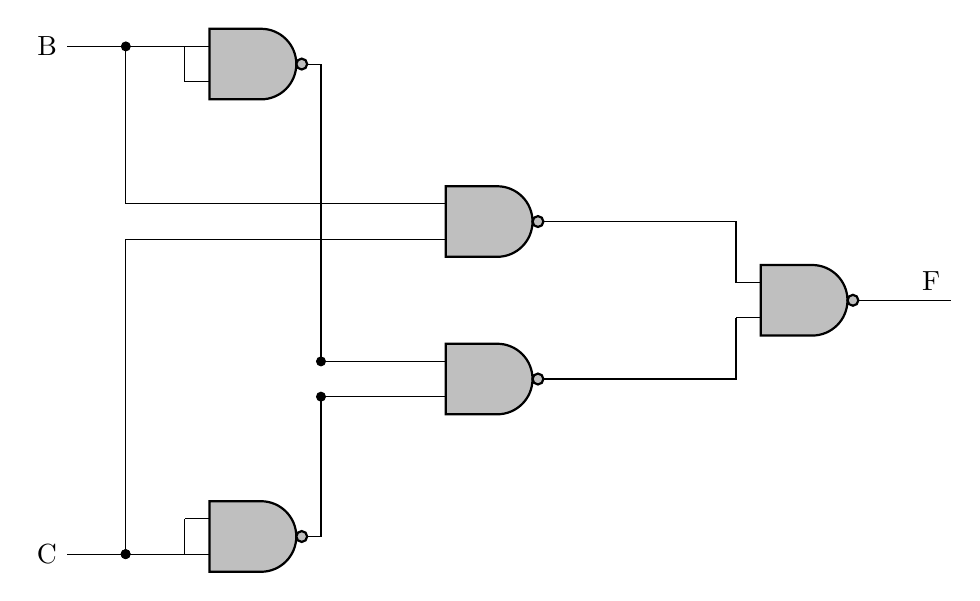
\begin{tikzpicture}
% Circuit style
\ctikzset{
    logic ports=ieee,
    logic ports/scale=0.8,
    logic ports/fill=lightgray
}
% Logic ports
\draw (3,0) node[nand port] (Nandb){};
\draw (3,-6) node[nand port] (Nandc){}; 
\draw (6,-2) node[nand port] (Nande){};
\draw (6,-4) node[nand port] (Nandf){};
\draw (10,-3) node[nand port] (Nandg){};
\draw (Nandg.out) -- ++(1,0) node[near end,above]{F};
% Connect NAND Gates
\draw (Nandb.in 1)--(Nandb.in 2);
\draw (Nandc.in 1)--(Nandc.in 2);
% Inputs
\draw (Nandb.in 1) -- ++(-1.5,0)node[left](In1){B};
\draw (Nandc.in 2) -- ++(-1.5,0)node[left](In2){C};
%Connection
\draw (In1)++(1,0) node [circ](x){};
\draw (In2) ++(1,0) node [circ](y){};
\draw (Nande.in 1) -| (x) ; 
\draw (Nande.in 2) -| (y)  node [circ]{} ;
\draw (Nandf.in 1) -|  node [circ]{}(Nandb.out) ; 
\draw (Nandf.in 2) -|  node [circ]{}(Nandc.out) ; 
\draw (Nande.out) -| (Nandg.in 1);
\draw (Nandf.out) -| (Nandg.in 2);
\end{tikzpicture}
\caption{NAND gate implementation for F}
\end{figure}
\end{document}